\subsubsection{Molecular Brain Cell Biology - IGF Binding Proteins}
\index{K�hl, Nicole}



\paragraph{Research Team}
Nicole K�hl (Research Instructor for Biochemistry and Cell Biology), Katja Laskowski (Lab Technician)\\


Multiple sclerosis (MS) to date is a non-curable neurological disorder with a prevalence of about 1:1000 in northern hemisphere states. Motoric dysfunctions that develop during the course of the disease arise after selective damage and loss of oligodendrocytes - the myelinating cells in the brain and spinal cord. The cause of MS remains elusive but it is believed that symptoms of MS arise partially due to auto-immune-mediated damage to the brain. In addition, it has long been known that IGF-1 is a crucial growth and survival factor for neurons as well as for oligodendrocytes. Therefore, IGF-1 is under intense investigation for its potential use as a restorative treatment for MS patients as well as patients suffering from other neurodegenerative diseases.

Our major research focus is molecular cell biology of brain glial
cells related to MS. One area of focus are cellular processes that
are related to the role of IGF-1 (insulin-like growth factor-1) in
the brain. We try to elucidate the regulation and function of a
network of IGF-binding proteins that modulate IGF-1 transport and
bioavailability which are important concerns for therapeutic use.


\paragraph{Highlights}
%
Additionally, a new focus of our work is the inter-cellular communication of microglial cells and oligodendrocytes. The widely accepted hypothesis for etiology of MS assumes that after disease-initiation and the development of inflammatory lesions, damage and loss of oligodendrocyte occur as a bystander effect due to activation of immune cells and due to the production of inflammatory mediators like NO, reactive oxygen species, and cytokines. Therefore, we have established co-culture systems consisting of purified primary rat microglia and oligodendrocytes to investigate the consequences of the cellular interplay under physiological as well as pathological conditions. The goal is to analyze the potential of IGF-1 to act as an immune-modulating agent.

Furthermore, we investigate the contribution of glial cells to antigen presentation after induced inflammation in a collaboration with Prof. Springer. Here, we are most interested in antigen presentation by the constitutive MHC class I molecules, as most glial cells are not true antigen presenting cells but have to be challenged to take up such a function.

Last, in collaboration with the lab of Prof. Brix we are trying to elucidate the role of cathepsin K in the mouse brain. The established K knockout mouse has a neurobehavioral phenotype that we investigated in the past. Now, we want to examine the underlying molecular network that results in the behavioral outcome.


\begin{figure}[ht]
  \begin{center}
   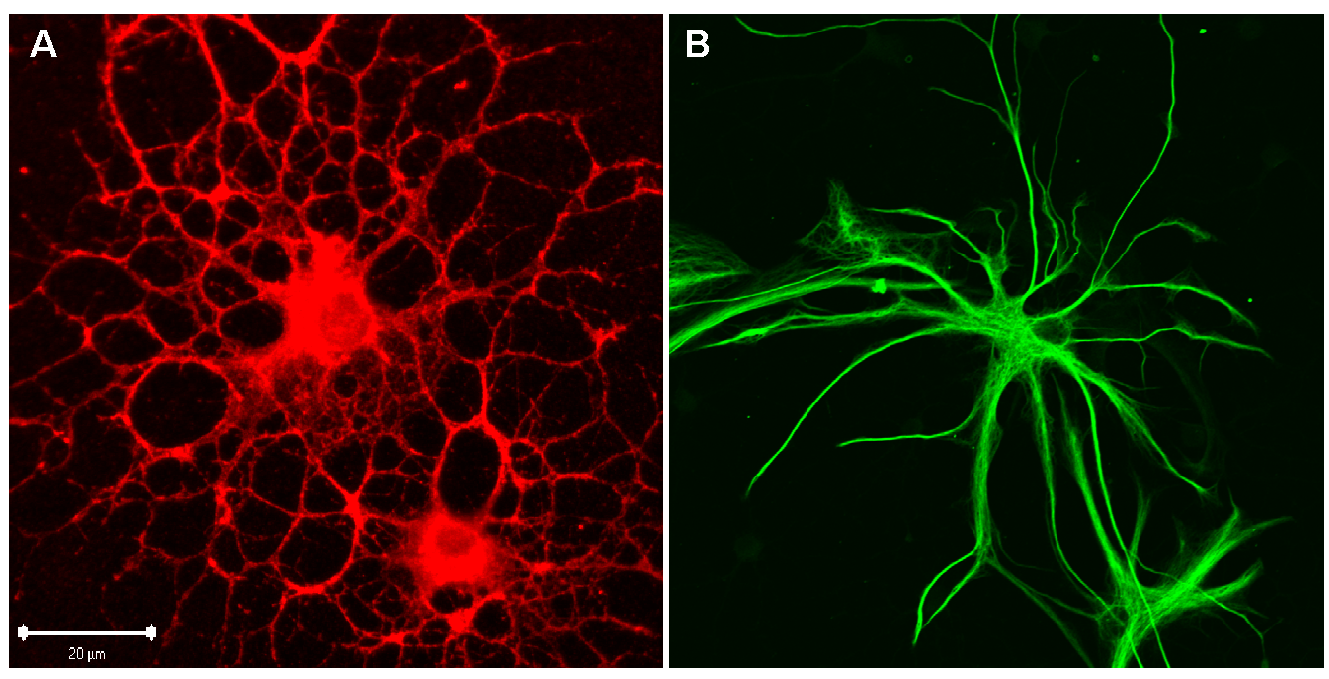
\includegraphics[width=\hsize]{Kuehl/Kuehl-fig1.pdf}
    \mycaption{Primary rat glial cells in culture A) Oligodendrocytes stained for CNPase; B) Astrocytes stained for GFAP. }\label{fig:Kuehl}
   \end{center}
\end{figure}

 
\myparagraph{Collaborations} Bremen Area Collaborations:
\begin{enumerate}
\item {\sl International University Bremen} \\ Prof. K. Brix \\ Brain proteases in health and disease
 \\ Prof. S. Springer \\ MHC class I and HLG expression in the
brain
\end{enumerate}
National \& International Collaborations:
\begin{enumerate}
\item {\sl Academic Hospital Groningen, The Netherlands} \\ Prof. J.H.A. De Keyser \\ Implications of IGF-binding proteins for MS therapy
\item {\sl Loma Linda Kidney Institute, CA, USA} \\ Dr. Donna Strong \\  IGFBP-6 trafficking in the cell
\end{enumerate}
